\SourceLeaf{213}\Needspace{20\baselineskip}
6. \emph{Lehrsatz.} Eine Gerade $CL\mathinner{.\,.\,.}$ oder $3$, die sich zwischen zwei Parallelen $AM\mathinner{.\,.\,.}$ oder $1$, $BN\mathinner{.\,.\,.}$ oder $2$ befindet, und keine von beiden schneidet, ist mit denselben parallel.

\textls{Beweis.} Man ziehe durch einen beliebigen Punkt $C$ in der Geraden $3$

\begin{center}
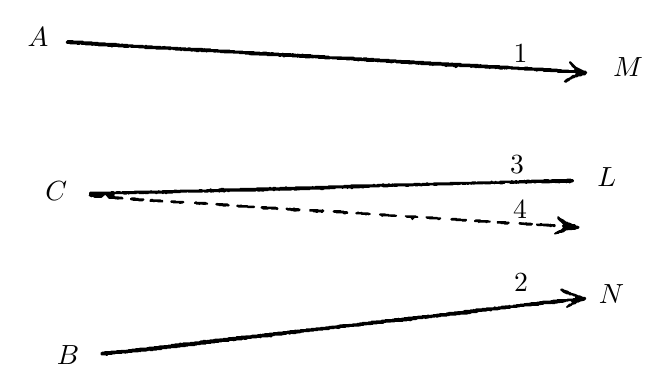
\begin{tikzpicture}[x=0.00656000cm,y=-0.00656000cm]
\fill[even odd rule] (1104,538) -- (1102,536) -- (1098,536) -- (1092,533) -- (1089,533) -- (1083,530) -- (1075,528) -- (1073,526) -- (1071,526) -- (1069,524) -- (1062,522) -- (1059,520) -- (1055,520) -- (1054,521) -- (1054,523) -- (1060,528) -- (1067,531) -- (1070,531) -- (1072,533) -- (1077,533) -- (1080,535) -- (1082,535) -- (1083,537) -- (1082,538) -- (1079,538) -- (1078,539) -- (1068,539) -- (1067,540) -- (1048,540) -- (1047,541) -- (1040,541) -- (1039,542) -- (1036,542) -- (1035,543) -- (1020,543) -- (1019,544) -- (1014,544) -- (1013,545) -- (1009,545) -- (1008,546) -- (997,546) -- (996,547) -- (984,548) -- (983,549) -- (976,549) -- (975,550) -- (969,550) -- (968,551) -- (963,551) -- (962,552) -- (957,552) -- (955,551) -- (954,552) -- (940,553) -- (939,554) -- (934,554) -- (933,555) -- (929,555) -- (927,554) -- (924,556) -- (911,556) -- (910,557) -- (903,557) -- (902,558) -- (891,558) -- (889,560) -- (886,559) -- (885,560) -- (880,560) -- (879,561) -- (869,561) -- (865,563) -- (849,564) -- (848,565) -- (838,565) -- (837,566) -- (834,566) -- (833,567) -- (821,567) -- (820,568) -- (815,568) -- (814,569) -- (808,569) -- (807,570) -- (804,570) -- (803,571) -- (797,570) -- (796,571) -- (787,571) -- (786,572) -- (778,572) -- (777,573) -- (769,573) -- (768,574) -- (759,574) -- (758,575) -- (752,575) -- (751,576) -- (747,576) -- (746,577) -- (742,577) -- (740,576) -- (739,577) -- (733,577) -- (732,578) -- (729,578) -- (728,579) -- (715,579) -- (714,580) -- (708,580) -- (707,581) -- (688,582) -- (687,583) -- (683,583) -- (682,584) -- (671,584) -- (670,585) -- (666,585) -- (665,586) -- (661,586) -- (660,587) -- (652,587) -- (651,588) -- (627,589) -- (626,590) -- (623,590) -- (622,591) -- (606,592) -- (605,593) -- (600,593) -- (599,594) -- (590,594) -- (589,595) -- (581,595) -- (580,596) -- (572,596) -- (571,597) -- (562,597) -- (561,598) -- (551,598) -- (550,599) -- (545,599) -- (544,600) -- (542,599) -- (540,599) -- (539,600) -- (531,600) -- (530,601) -- (526,601) -- (525,602) -- (517,602) -- (516,603) -- (507,603) -- (506,604) -- (499,604) -- (498,605) -- (491,605) -- (490,606) -- (482,606) -- (481,607) -- (477,607) -- (476,608) -- (473,607) -- (472,608) -- (468,608) -- (467,609) -- (457,609) -- (456,610) -- (436,611) -- (435,612) -- (427,612) -- (426,613) -- (411,614) -- (410,615) -- (402,615) -- (401,616) -- (383,617) -- (382,618) -- (376,618) -- (375,619) -- (370,619) -- (369,620) -- (367,619) -- (363,619) -- (362,620) -- (358,620) -- (354,622) -- (346,622) -- (345,623) -- (338,623) -- (337,624) -- (324,624) -- (323,625) -- (320,625) -- (318,624) -- (315,626) -- (308,626) -- (307,627) -- (301,627) -- (300,628) -- (295,628) -- (294,629) -- (277,630) -- (276,631) -- (268,631) -- (267,632) -- (258,632) -- (257,633) -- (254,633) -- (253,634) -- (240,634) -- (239,635) -- (232,635) -- (231,636) -- (225,636) -- (224,637) -- (218,637) -- (217,638) -- (195,639) -- (194,640) -- (184,640) -- (183,641) -- (172,641) -- (171,642) -- (167,642) -- (164,644) -- (164,647) -- (166,649) -- (174,649) -- (175,650) -- (177,650) -- (179,648) -- (186,648) -- (187,647) -- (192,647) -- (193,646) -- (205,646) -- (206,645) -- (210,645) -- (212,646) -- (213,645) -- (217,645) -- (218,644) -- (225,644) -- (226,643) -- (237,643) -- (238,642) -- (241,643) -- (242,642) -- (252,642) -- (253,641) -- (256,641) -- (257,640) -- (259,640) -- (260,641) -- (265,641) -- (266,640) -- (272,640) -- (273,639) -- (281,639) -- (284,637) -- (292,637) -- (293,636) -- (300,636) -- (301,635) -- (312,635) -- (313,634) -- (318,634) -- (319,633) -- (328,633) -- (329,632) -- (333,632) -- (334,631) -- (346,631) -- (347,630) -- (350,630) -- (351,629) -- (357,629) -- (358,628) -- (368,628) -- (369,627) -- (377,627) -- (378,626) -- (385,626) -- (386,625) -- (392,625) -- (393,624) -- (398,624) -- (399,623) -- (412,623) -- (414,621) -- (420,621) -- (422,622) -- (423,621) -- (426,621) -- (427,620) -- (437,620) -- (440,618) -- (442,619) -- (446,619) -- (450,617) -- (456,617) -- (457,616) -- (466,616) -- (467,615) -- (472,615) -- (474,616) -- (476,614) -- (489,614) -- (490,613) -- (492,614) -- (495,614) -- (497,612) -- (500,612) -- (501,611) -- (515,611) -- (516,610) -- (524,609) -- (525,608) -- (528,608) -- (530,609) -- (534,607) -- (536,608) -- (541,608) -- (542,607) -- (552,606) -- (553,605) -- (557,605) -- (558,604) -- (568,604) -- (569,603) -- (576,603) -- (577,602) -- (584,602) -- (585,601) -- (594,601) -- (595,600) -- (606,600) -- (609,598) -- (616,598) -- (617,597) -- (625,598) -- (629,596) -- (638,596) -- (639,595) -- (645,595) -- (646,594) -- (667,593) -- (668,592) -- (673,592) -- (674,591) -- (691,590) -- (692,589) -- (699,589) -- (700,588) -- (711,588) -- (714,586) -- (733,585) -- (734,584) -- (749,584) -- (750,583) -- (757,583) -- (758,582) -- (764,583) -- (768,581) -- (774,581) -- (778,579) -- (787,579) -- (788,578) -- (792,578) -- (794,579) -- (795,578) -- (798,578) -- (799,577) -- (805,577) -- (806,576) -- (811,576) -- (812,575) -- (814,576) -- (817,576) -- (818,575) -- (822,575) -- (823,574) -- (834,574) -- (835,573) -- (839,573) -- (840,572) -- (852,572) -- (853,571) -- (860,571) -- (861,570) -- (874,570) -- (875,569) -- (879,569) -- (883,567) -- (892,567) -- (896,565) -- (912,564) -- (913,563) -- (917,563) -- (918,564) -- (920,564) -- (922,562) -- (933,562) -- (934,561) -- (937,561) -- (938,560) -- (948,560) -- (949,559) -- (956,559) -- (960,557) -- (970,557) -- (971,556) -- (975,556) -- (976,555) -- (984,555) -- (985,554) -- (998,554) -- (999,553) -- (1012,553) -- (1013,552) -- (1021,551) -- (1022,550) -- (1036,550) -- (1037,549) -- (1039,550) -- (1043,550) -- (1044,549) -- (1048,549) -- (1049,548) -- (1061,547) -- (1062,546) -- (1064,546) -- (1065,545) -- (1069,545) -- (1070,544) -- (1074,544) -- (1076,546) -- (1076,547) -- (1074,549) -- (1071,549) -- (1065,555) -- (1065,556) -- (1067,557) -- (1076,553) -- (1078,551) -- (1083,550) -- (1086,547) -- (1089,547) -- (1092,545) -- (1101,543) -- (1104,540) -- cycle
(1007,395) -- (1007,397) -- (1011,399) -- (1017,399) -- (1019,398) -- (1020,399) -- (1033,400) -- (1034,401) -- (1036,401) -- (1037,400) -- (1040,400) -- (1042,401) -- (1045,399) -- (1045,397) -- (1043,395) -- (1036,395) -- (1035,394) -- (1032,395) -- (1031,394) -- (1019,394) -- (1018,393) -- (1015,393) -- (1014,394) -- (1008,394) -- cycle
(973,393) -- (973,394) -- (975,396) -- (987,397) -- (988,398) -- (998,398) -- (1001,395) -- (1000,393) -- (998,393) -- (997,392) -- (989,392) -- (988,391) -- (986,392) -- (975,391) -- cycle
(931,390) -- (931,393) -- (932,394) -- (938,394) -- (939,395) -- (945,395) -- (946,396) -- (952,396) -- (956,393) -- (956,392) -- (954,390) -- (949,390) -- (948,389) -- (932,389) -- cycle
(887,388) -- (887,390) -- (888,391) -- (894,391) -- (896,393) -- (898,392) -- (909,392) -- (910,393) -- (912,393) -- (913,392) -- (918,392) -- (919,391) -- (919,389) -- (918,388) -- (915,388) -- (914,387) -- (900,387) -- (899,386) -- (890,386) -- cycle
(841,385) -- (841,386) -- (843,388) -- (851,388) -- (852,389) -- (863,389) -- (864,390) -- (871,390) -- (873,388) -- (873,386) -- (872,385) -- (862,385) -- (861,384) -- (854,384) -- (853,383) -- (844,383) -- cycle
(1042,414) -- (1043,415) -- (1046,415) -- (1047,414) -- (1050,414) -- (1053,412) -- (1057,412) -- (1058,411) -- (1060,411) -- (1065,407) -- (1083,406) -- (1084,405) -- (1089,404) -- (1091,402) -- (1091,400) -- (1087,398) -- (1085,398) -- (1082,395) -- (1078,395) -- (1072,392) -- (1070,392) -- (1067,390) -- (1065,390) -- (1060,386) -- (1054,383) -- (1051,380) -- (1049,380) -- (1048,381) -- (1048,384) -- (1049,386) -- (1059,395) -- (1059,396) -- (1057,398) -- (1059,402) -- (1055,406) -- (1051,407) -- (1044,411) -- (1042,413) -- cycle
(793,381) -- (793,382) -- (796,385) -- (800,385) -- (801,386) -- (816,386) -- (817,387) -- (820,387) -- (823,385) -- (823,383) -- (822,382) -- (817,382) -- (816,381) -- (808,381) -- (807,380) -- (794,380) -- cycle
(753,379) -- (753,380) -- (757,383) -- (764,383) -- (767,387) -- (768,387) -- (772,383) -- (778,383) -- (779,382) -- (779,381) -- (777,379) -- (775,379) -- (774,378) -- (754,378) -- cycle
(703,376) -- (704,378) -- (707,379) -- (709,381) -- (711,380) -- (721,380) -- (722,381) -- (724,380) -- (726,381) -- (736,381) -- (738,379) -- (737,377) -- (735,377) -- (734,376) -- (722,376) -- (721,375) -- (716,375) -- (715,374) -- (705,374) -- cycle
(657,373) -- (657,374) -- (659,376) -- (668,376) -- (669,377) -- (676,377) -- (677,378) -- (679,378) -- (680,377) -- (683,378) -- (687,376) -- (687,375) -- (685,373) -- (683,373) -- (682,372) -- (671,372) -- (670,371) -- (665,372) -- (664,371) -- (661,371) -- cycle
(613,370) -- (614,372) -- (616,373) -- (619,373) -- (620,374) -- (632,374) -- (635,376) -- (638,376) -- (639,375) -- (642,375) -- (643,374) -- (643,372) -- (641,370) -- (636,370) -- (635,369) -- (630,369) -- (629,368) -- (616,368) -- cycle
(568,367) -- (568,370) -- (569,371) -- (575,371) -- (576,372) -- (580,372) -- (581,373) -- (584,373) -- (585,372) -- (590,372) -- (591,373) -- (594,373) -- (597,370) -- (597,369) -- (594,366) -- (592,367) -- (586,367) -- (585,366) -- (569,366) -- cycle
(522,365) -- (523,367) -- (527,369) -- (532,369) -- (533,370) -- (537,370) -- (538,371) -- (549,370) -- (551,368) -- (551,366) -- (550,365) -- (548,365) -- (547,364) -- (541,364) -- (540,363) -- (537,363) -- (536,364) -- (532,364) -- (531,363) -- (527,364) -- (526,363) -- (524,363) -- cycle
(474,362) -- (474,364) -- (479,367) -- (488,367) -- (489,366) -- (494,366) -- (495,367) -- (504,367) -- (506,368) -- (508,366) -- (508,364) -- (506,362) -- (504,362) -- (503,361) -- (486,361) -- (485,360) -- (476,360) -- cycle
(427,359) -- (427,361) -- (431,363) -- (448,363) -- (449,364) -- (461,364) -- (463,362) -- (463,361) -- (461,359) -- (449,359) -- (448,358) -- (438,358) -- (437,357) -- (434,357) -- (433,358) -- (429,357) -- cycle
(386,356) -- (386,357) -- (389,359) -- (392,359) -- (393,360) -- (400,360) -- (401,361) -- (407,361) -- (408,360) -- (411,361) -- (414,359) -- (414,358) -- (410,355) -- (389,354) -- cycle
(345,353) -- (345,355) -- (346,356) -- (348,356) -- (349,357) -- (354,357) -- (355,358) -- (357,357) -- (367,358) -- (368,357) -- (371,357) -- (372,356) -- (372,355) -- (370,353) -- (368,353) -- (367,352) -- (351,352) -- (350,351) -- (348,351) -- cycle
(299,351) -- (299,352) -- (301,354) -- (304,354) -- (305,355) -- (316,355) -- (317,356) -- (323,355) -- (326,353) -- (326,352) -- (324,350) -- (310,350) -- (309,349) -- (301,349) -- cycle
(259,348) -- (259,351) -- (260,352) -- (266,352) -- (267,353) -- (269,352) -- (274,352) -- (275,353) -- (284,353) -- (285,352) -- (285,349) -- (284,348) -- (281,348) -- (280,347) -- (266,347) -- (265,346) -- (261,346) -- cycle
(221,345) -- (221,347) -- (223,349) -- (226,349) -- (227,350) -- (237,350) -- (238,351) -- (245,351) -- (249,348) -- (249,347) -- (247,345) -- (238,345) -- (237,344) -- (232,344) -- (231,343) -- (225,343) -- cycle
(1080,310) -- (1078,308) -- (1075,308) -- (1074,307) -- (1067,307) -- (1066,308) -- (1037,308) -- (1036,309) -- (1032,309) -- (1031,308) -- (1022,308) -- (1021,309) -- (998,309) -- (997,310) -- (995,310) -- (994,309) -- (989,309) -- (988,310) -- (986,310) -- (984,309) -- (983,310) -- (974,310) -- (973,311) -- (971,311) -- (970,310) -- (967,310) -- (966,311) -- (962,311) -- (961,310) -- (959,310) -- (958,311) -- (937,311) -- (936,312) -- (930,312) -- (929,311) -- (927,312) -- (923,312) -- (922,311) -- (920,311) -- (919,312) -- (894,312) -- (893,313) -- (891,313) -- (890,312) -- (883,312) -- (882,313) -- (841,313) -- (840,314) -- (809,314) -- (808,315) -- (798,315) -- (797,314) -- (795,314) -- (794,315) -- (787,315) -- (786,316) -- (783,316) -- (782,315) -- (771,315) -- (770,316) -- (732,316) -- (731,317) -- (729,316) -- (727,317) -- (724,317) -- (723,316) -- (721,316) -- (720,317) -- (713,317) -- (712,316) -- (710,316) -- (709,317) -- (700,317) -- (699,318) -- (695,318) -- (694,317) -- (692,317) -- (691,318) -- (649,318) -- (648,319) -- (635,319) -- (634,320) -- (605,320) -- (604,321) -- (580,321) -- (579,322) -- (576,322) -- (575,321) -- (573,322) -- (541,322) -- (540,323) -- (525,323) -- (524,322) -- (522,322) -- (521,323) -- (511,323) -- (510,324) -- (504,324) -- (503,323) -- (498,323) -- (497,324) -- (494,324) -- (493,323) -- (491,323) -- (490,324) -- (466,324) -- (465,325) -- (434,325) -- (433,326) -- (403,326) -- (402,325) -- (397,325) -- (396,326) -- (393,326) -- (392,327) -- (379,327) -- (378,326) -- (376,326) -- (375,327) -- (370,327) -- (369,328) -- (361,328) -- (360,327) -- (355,327) -- (354,328) -- (318,328) -- (317,329) -- (307,328) -- (306,329) -- (284,329) -- (283,330) -- (278,330) -- (277,329) -- (275,330) -- (263,330) -- (262,329) -- (260,330) -- (230,330) -- (229,331) -- (206,331) -- (205,332) -- (203,332) -- (202,331) -- (195,331) -- (194,332) -- (190,332) -- (189,331) -- (185,331) -- (184,332) -- (144,332) -- (142,334) -- (142,338) -- (141,340) -- (146,343) -- (149,342) -- (152,344) -- (166,344) -- (172,339) -- (174,339) -- (180,346) -- (191,346) -- (192,347) -- (196,347) -- (198,348) -- (199,347) -- (207,347) -- (208,346) -- (208,344) -- (206,342) -- (192,341) -- (190,339) -- (192,337) -- (208,337) -- (209,338) -- (214,338) -- (215,337) -- (217,337) -- (218,338) -- (220,337) -- (233,337) -- (234,336) -- (238,336) -- (239,337) -- (248,337) -- (249,336) -- (251,337) -- (256,337) -- (257,336) -- (270,336) -- (271,337) -- (273,337) -- (274,336) -- (283,336) -- (285,337) -- (286,336) -- (289,336) -- (290,337) -- (292,337) -- (293,336) -- (303,336) -- (304,335) -- (318,335) -- (319,334) -- (331,334) -- (332,333) -- (334,334) -- (361,334) -- (362,333) -- (364,333) -- (365,334) -- (372,334) -- (373,333) -- (376,333) -- (377,334) -- (379,334) -- (380,333) -- (382,334) -- (384,333) -- (392,333) -- (394,334) -- (395,333) -- (401,333) -- (403,334) -- (407,332) -- (409,332) -- (410,333) -- (413,333) -- (414,332) -- (464,332) -- (465,331) -- (467,331) -- (468,332) -- (473,332) -- (474,331) -- (476,332) -- (480,332) -- (481,331) -- (488,331) -- (489,330) -- (497,330) -- (498,331) -- (501,331) -- (502,330) -- (508,330) -- (510,331) -- (511,330) -- (533,330) -- (534,329) -- (538,329) -- (539,330) -- (544,330) -- (546,329) -- (548,330) -- (549,329) -- (569,329) -- (570,328) -- (589,328) -- (590,329) -- (595,329) -- (596,328) -- (618,327) -- (619,326) -- (631,326) -- (632,327) -- (634,326) -- (641,326) -- (642,327) -- (643,326) -- (648,326) -- (649,327) -- (652,327) -- (653,326) -- (665,326) -- (666,325) -- (673,326) -- (674,325) -- (684,325) -- (685,324) -- (703,324) -- (706,322) -- (710,323) -- (711,324) -- (720,324) -- (721,323) -- (730,323) -- (731,322) -- (732,323) -- (738,323) -- (739,322) -- (754,322) -- (755,323) -- (760,323) -- (761,322) -- (769,322) -- (770,321) -- (772,321) -- (773,322) -- (778,322) -- (779,321) -- (786,322) -- (787,321) -- (800,321) -- (801,320) -- (808,320) -- (809,321) -- (815,321) -- (816,320) -- (846,320) -- (847,319) -- (854,319) -- (856,320) -- (857,319) -- (860,319) -- (861,318) -- (863,318) -- (864,319) -- (871,319) -- (872,318) -- (874,319) -- (876,319) -- (877,318) -- (880,318) -- (881,319) -- (885,318) -- (887,319) -- (888,318) -- (905,318) -- (906,317) -- (908,318) -- (919,318) -- (920,317) -- (925,317) -- (926,318) -- (928,317) -- (936,317) -- (937,318) -- (942,318) -- (943,317) -- (946,317) -- (948,315) -- (956,316) -- (957,317) -- (965,317) -- (966,316) -- (968,317) -- (970,317) -- (971,316) -- (973,317) -- (975,316) -- (986,316) -- (987,317) -- (989,317) -- (990,316) -- (998,316) -- (999,315) -- (1002,315) -- (1003,316) -- (1007,316) -- (1008,315) -- (1017,315) -- (1018,316) -- (1033,316) -- (1034,315) -- (1036,316) -- (1038,315) -- (1053,316) -- (1054,315) -- (1064,315) -- (1066,316) -- (1067,315) -- (1070,315) -- (1071,316) -- (1073,316) -- (1074,315) -- (1078,314) -- (1080,312) -- cycle
(97,42) -- (97,44) -- (99,46) -- (104,46) -- (105,47) -- (118,47) -- (119,48) -- (123,48) -- (124,47) -- (126,47) -- (127,48) -- (134,48) -- (135,49) -- (146,49) -- (147,50) -- (152,49) -- (153,50) -- (159,50) -- (160,51) -- (177,51) -- (178,52) -- (184,52) -- (185,53) -- (187,53) -- (188,52) -- (197,52) -- (198,53) -- (208,53) -- (209,54) -- (218,54) -- (219,53) -- (222,53) -- (223,54) -- (237,54) -- (238,55) -- (249,55) -- (250,56) -- (270,56) -- (271,57) -- (295,57) -- (296,58) -- (300,58) -- (301,57) -- (303,57) -- (304,58) -- (308,58) -- (309,59) -- (318,59) -- (319,60) -- (321,60) -- (322,59) -- (324,59) -- (325,60) -- (338,60) -- (339,61) -- (342,61) -- (344,60) -- (345,61) -- (348,61) -- (349,62) -- (354,62) -- (355,61) -- (358,61) -- (359,62) -- (368,62) -- (369,63) -- (371,62) -- (382,62) -- (383,63) -- (387,63) -- (389,62) -- (390,63) -- (395,63) -- (396,64) -- (432,65) -- (433,66) -- (443,66) -- (444,67) -- (451,67) -- (452,68) -- (486,69) -- (487,70) -- (508,70) -- (509,71) -- (513,71) -- (515,70) -- (518,72) -- (520,72) -- (521,71) -- (534,71) -- (535,72) -- (544,72) -- (545,73) -- (548,72) -- (549,73) -- (559,73) -- (560,74) -- (570,74) -- (571,73) -- (573,74) -- (576,74) -- (578,73) -- (579,74) -- (585,74) -- (586,75) -- (597,75) -- (598,76) -- (608,76) -- (609,75) -- (611,75) -- (612,76) -- (621,76) -- (622,77) -- (639,77) -- (640,78) -- (646,78) -- (648,77) -- (649,78) -- (653,78) -- (654,79) -- (661,79) -- (662,80) -- (664,80) -- (665,79) -- (678,80) -- (679,81) -- (693,81) -- (695,80) -- (696,81) -- (699,81) -- (700,82) -- (704,81) -- (705,82) -- (716,82) -- (717,83) -- (725,83) -- (726,84) -- (734,82) -- (737,84) -- (745,84) -- (746,85) -- (760,85) -- (761,86) -- (773,85) -- (774,86) -- (778,86) -- (779,87) -- (781,86) -- (783,86) -- (784,87) -- (799,87) -- (800,88) -- (806,88) -- (807,89) -- (809,88) -- (824,88) -- (825,89) -- (829,89) -- (833,91) -- (835,90) -- (846,90) -- (847,91) -- (849,91) -- (851,93) -- (854,92) -- (856,90) -- (858,90) -- (859,91) -- (879,91) -- (881,93) -- (883,92) -- (888,92) -- (889,93) -- (892,93) -- (893,92) -- (895,93) -- (907,93) -- (908,94) -- (916,94) -- (917,95) -- (919,94) -- (927,94) -- (928,95) -- (932,94) -- (933,95) -- (936,95) -- (937,96) -- (942,96) -- (943,95) -- (945,95) -- (946,96) -- (948,95) -- (950,96) -- (952,95) -- (958,95) -- (959,96) -- (971,96) -- (972,97) -- (984,97) -- (985,98) -- (1003,98) -- (1004,99) -- (1007,99) -- (1008,100) -- (1010,99) -- (1020,99) -- (1021,100) -- (1048,101) -- (1049,102) -- (1082,102) -- (1084,104) -- (1082,106) -- (1078,106) -- (1072,111) -- (1065,114) -- (1061,118) -- (1061,119) -- (1063,121) -- (1066,121) -- (1068,119) -- (1071,118) -- (1074,115) -- (1076,115) -- (1078,113) -- (1080,113) -- (1083,111) -- (1086,111) -- (1089,109) -- (1094,109) -- (1097,107) -- (1102,107) -- (1106,102) -- (1106,101) -- (1103,98) -- (1100,98) -- (1084,90) -- (1074,80) -- (1072,80) -- (1071,81) -- (1071,83) -- (1076,89) -- (1076,90) -- (1081,94) -- (1081,96) -- (1080,97) -- (1071,97) -- (1070,96) -- (1057,96) -- (1056,95) -- (1049,95) -- (1048,94) -- (1037,94) -- (1036,93) -- (1022,93) -- (1021,92) -- (1000,92) -- (999,91) -- (992,91) -- (991,90) -- (985,90) -- (984,91) -- (975,91) -- (974,90) -- (962,90) -- (961,89) -- (958,90) -- (957,89) -- (954,89) -- (953,88) -- (937,88) -- (936,87) -- (914,87) -- (913,86) -- (901,86) -- (900,85) -- (896,86) -- (895,85) -- (862,84) -- (861,83) -- (846,83) -- (845,82) -- (839,83) -- (838,82) -- (824,82) -- (823,81) -- (804,81) -- (803,80) -- (790,80) -- (789,79) -- (772,79) -- (771,78) -- (737,77) -- (736,76) -- (723,76) -- (722,75) -- (705,75) -- (704,74) -- (693,74) -- (692,73) -- (687,73) -- (685,74) -- (684,73) -- (680,73) -- (679,72) -- (673,72) -- (672,73) -- (670,73) -- (669,72) -- (656,72) -- (655,71) -- (607,70) -- (606,69) -- (599,69) -- (598,68) -- (572,67) -- (571,66) -- (557,66) -- (556,65) -- (554,65) -- (553,66) -- (545,65) -- (543,66) -- (542,65) -- (538,65) -- (537,64) -- (535,64) -- (534,65) -- (532,64) -- (518,64) -- (517,63) -- (515,64) -- (510,64) -- (509,63) -- (499,63) -- (498,62) -- (494,62) -- (492,63) -- (491,62) -- (486,62) -- (485,61) -- (478,61) -- (477,62) -- (473,62) -- (472,61) -- (462,61) -- (461,60) -- (440,60) -- (439,59) -- (424,59) -- (423,58) -- (415,58) -- (414,57) -- (392,57) -- (391,56) -- (378,56) -- (377,55) -- (366,55) -- (365,54) -- (363,55) -- (361,54) -- (339,54) -- (338,53) -- (333,53) -- (332,54) -- (330,54) -- (329,53) -- (320,53) -- (319,52) -- (315,53) -- (314,52) -- (301,52) -- (300,51) -- (290,51) -- (289,50) -- (281,51) -- (280,50) -- (265,50) -- (264,49) -- (254,49) -- (253,48) -- (251,48) -- (250,49) -- (247,49) -- (246,48) -- (228,48) -- (227,47) -- (217,47) -- (216,46) -- (207,46) -- (206,45) -- (204,46) -- (201,46) -- (200,45) -- (195,45) -- (194,44) -- (174,44) -- (173,43) -- (160,43) -- (159,42) -- (148,42) -- (147,41) -- (131,41) -- (130,40) -- (112,40) -- (111,39) -- (100,39) -- cycle;
\node[inner sep=0pt] at (43,33) {$A$};
\node[inner sep=0pt] at (977,64) {$1$};
\node[inner sep=0pt] at (1185,91) {$M$};
\node[inner sep=0pt] at (970,280) {$3$};
\node[inner sep=0pt] at (1144,303) {$L$};
\node[inner sep=0pt] at (78,330) {$C$};
\node[inner sep=0pt] at (976,366) {$4$};
\node[inner sep=0pt] at (978,508) {$2$};
\node[inner sep=0pt] at (1153,531) {$N$};
\node[inner sep=0pt] at (101,648) {$B$};
\end{tikzpicture}

\end{center}
\noindent eine Parallele $4$ mit $2$; wäre diese von $3$ verschieden, so müsste $3$ entweder zwischen $1$ und $4$ oder zwischen $2$ und $4$ fallen; in jenem Fall würde sie (Definition der Parallelen) die $1$, im andern die $2$ schneiden müssen, gegen die Voraussetzung.

7. \emph{Lehrsatz.} Zwei Parallellinien, rückwärts fortgesetzt, können einander auf dieser Seite nicht schneiden.

\begin{center}
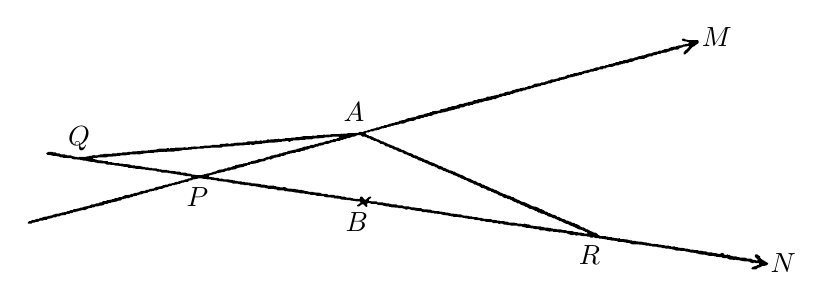
\begin{tikzpicture}[x=0.00610128cm,y=-0.00610128cm]
\fill[even odd rule] (1555,523) -- (1554,521) -- (1541,513) -- (1538,510) -- (1538,507) -- (1534,505) -- (1532,503) -- (1529,503) -- (1527,505) -- (1527,508) -- (1533,514) -- (1532,516) -- (1530,516) -- (1529,515) -- (1522,514) -- (1519,512) -- (1511,512) -- (1507,510) -- (1496,510) -- (1495,509) -- (1491,509) -- (1488,507) -- (1481,507) -- (1480,506) -- (1477,506) -- (1474,504) -- (1471,504) -- (1470,503) -- (1468,504) -- (1464,504) -- (1461,500) -- (1458,500) -- (1455,502) -- (1450,502) -- (1449,501) -- (1439,500) -- (1438,499) -- (1429,499) -- (1426,497) -- (1420,497) -- (1419,496) -- (1415,496) -- (1414,495) -- (1411,496) -- (1408,494) -- (1400,494) -- (1399,493) -- (1392,493) -- (1391,492) -- (1388,492) -- (1387,491) -- (1381,491) -- (1380,490) -- (1367,489) -- (1366,488) -- (1362,488) -- (1359,486) -- (1357,487) -- (1353,487) -- (1352,486) -- (1349,486) -- (1348,485) -- (1340,485) -- (1339,484) -- (1333,484) -- (1332,483) -- (1327,483) -- (1326,482) -- (1312,481) -- (1311,480) -- (1307,480) -- (1306,479) -- (1302,479) -- (1301,478) -- (1296,478) -- (1295,477) -- (1280,476) -- (1279,475) -- (1272,475) -- (1271,474) -- (1267,474) -- (1266,473) -- (1263,473) -- (1262,472) -- (1247,471) -- (1245,469) -- (1243,470) -- (1240,470) -- (1239,469) -- (1235,469) -- (1234,468) -- (1230,468) -- (1229,467) -- (1222,467) -- (1221,466) -- (1218,466) -- (1217,465) -- (1206,465) -- (1202,463) -- (1199,460) -- (1195,458) -- (1190,457) -- (1188,455) -- (1186,455) -- (1179,451) -- (1177,451) -- (1171,447) -- (1168,447) -- (1164,445) -- (1162,443) -- (1156,440) -- (1154,440) -- (1152,438) -- (1146,437) -- (1144,435) -- (1142,435) -- (1138,433) -- (1135,433) -- (1131,430) -- (1126,429) -- (1119,425) -- (1116,425) -- (1114,423) -- (1110,421) -- (1105,420) -- (1100,417) -- (1098,417) -- (1093,414) -- (1091,414) -- (1089,412) -- (1083,409) -- (1080,409) -- (1078,407) -- (1072,404) -- (1065,403) -- (1049,395) -- (1041,393) -- (1034,389) -- (1032,389) -- (1030,387) -- (1028,387) -- (1025,384) -- (1022,384) -- (1016,381) -- (1011,380) -- (1008,378) -- (1003,377) -- (1001,375) -- (999,375) -- (988,369) -- (986,369) -- (981,366) -- (979,366) -- (969,361) -- (967,361) -- (963,358) -- (960,358) -- (956,355) -- (951,354) -- (945,350) -- (942,350) -- (938,348) -- (936,346) -- (928,344) -- (918,338) -- (913,337) -- (911,335) -- (909,335) -- (905,333) -- (903,331) -- (900,331) -- (897,329) -- (891,328) -- (889,326) -- (887,326) -- (882,323) -- (879,323) -- (877,321) -- (873,319) -- (870,319) -- (866,316) -- (864,316) -- (859,313) -- (852,311) -- (845,307) -- (840,306) -- (838,304) -- (834,303) -- (831,301) -- (829,301) -- (822,297) -- (818,297) -- (816,295) -- (812,293) -- (805,291) -- (796,286) -- (791,285) -- (789,283) -- (787,283) -- (785,281) -- (779,280) -- (775,277) -- (773,277) -- (767,274) -- (765,274) -- (758,270) -- (756,270) -- (754,268) -- (751,268) -- (744,264) -- (742,264) -- (728,257) -- (725,257) -- (723,255) -- (721,255) -- (717,252) -- (717,251) -- (719,249) -- (724,249) -- (728,247) -- (733,247) -- (736,245) -- (741,245) -- (742,244) -- (744,244) -- (751,241) -- (754,241) -- (755,240) -- (760,240) -- (762,238) -- (769,237) -- (770,236) -- (776,235) -- (777,234) -- (785,233) -- (789,231) -- (796,231) -- (804,227) -- (807,227) -- (808,226) -- (811,226) -- (812,225) -- (817,225) -- (818,224) -- (820,224) -- (822,222) -- (830,221) -- (834,219) -- (837,219) -- (840,217) -- (845,217) -- (848,215) -- (854,215) -- (859,212) -- (865,211) -- (869,209) -- (874,209) -- (875,208) -- (883,207) -- (884,206) -- (887,206) -- (891,204) -- (895,204) -- (896,203) -- (902,202) -- (903,201) -- (906,201) -- (907,200) -- (912,200) -- (915,197) -- (920,197) -- (929,193) -- (932,194) -- (936,192) -- (940,192) -- (942,190) -- (945,190) -- (946,189) -- (951,189) -- (954,187) -- (958,187) -- (965,184) -- (974,183) -- (975,182) -- (978,182) -- (982,180) -- (988,180) -- (990,178) -- (992,178) -- (995,176) -- (998,176) -- (1004,173) -- (1009,173) -- (1012,171) -- (1017,171) -- (1020,169) -- (1023,169) -- (1030,166) -- (1033,166) -- (1037,164) -- (1042,164) -- (1045,162) -- (1049,162) -- (1052,160) -- (1059,159) -- (1062,157) -- (1065,157) -- (1069,155) -- (1073,155) -- (1074,154) -- (1081,153) -- (1083,151) -- (1091,150) -- (1098,147) -- (1103,147) -- (1106,145) -- (1112,144) -- (1115,142) -- (1120,142) -- (1123,140) -- (1131,139) -- (1132,138) -- (1134,138) -- (1141,135) -- (1144,135) -- (1145,134) -- (1148,134) -- (1149,133) -- (1152,133) -- (1153,132) -- (1156,132) -- (1157,131) -- (1160,131) -- (1161,130) -- (1166,130) -- (1168,128) -- (1170,128) -- (1173,126) -- (1179,126) -- (1185,123) -- (1190,123) -- (1194,121) -- (1198,121) -- (1204,118) -- (1210,118) -- (1212,116) -- (1217,116) -- (1219,114) -- (1222,114) -- (1223,113) -- (1230,113) -- (1237,110) -- (1243,110) -- (1245,108) -- (1248,108) -- (1249,107) -- (1252,107) -- (1253,106) -- (1256,106) -- (1257,105) -- (1263,105) -- (1265,103) -- (1273,102) -- (1278,99) -- (1281,99) -- (1285,97) -- (1292,97) -- (1293,96) -- (1297,96) -- (1299,94) -- (1301,94) -- (1307,91) -- (1313,91) -- (1315,89) -- (1322,88) -- (1325,86) -- (1330,86) -- (1333,84) -- (1336,84) -- (1337,83) -- (1343,83) -- (1346,81) -- (1349,81) -- (1352,79) -- (1355,79) -- (1359,77) -- (1367,77) -- (1369,75) -- (1373,73) -- (1375,73) -- (1378,71) -- (1382,71) -- (1383,70) -- (1386,70) -- (1387,69) -- (1389,69) -- (1390,70) -- (1390,72) -- (1388,73) -- (1387,75) -- (1384,78) -- (1383,78) -- (1379,83) -- (1379,86) -- (1380,87) -- (1382,87) -- (1385,84) -- (1386,84) -- (1398,71) -- (1401,70) -- (1404,67) -- (1407,66) -- (1410,63) -- (1410,59) -- (1408,57) -- (1387,57) -- (1386,56) -- (1383,56) -- (1380,54) -- (1377,54) -- (1375,56) -- (1375,57) -- (1377,59) -- (1379,59) -- (1380,60) -- (1385,60) -- (1386,61) -- (1389,61) -- (1390,63) -- (1388,65) -- (1383,65) -- (1382,66) -- (1379,66) -- (1375,68) -- (1369,68) -- (1368,69) -- (1365,69) -- (1362,71) -- (1357,71) -- (1356,72) -- (1353,72) -- (1352,73) -- (1350,73) -- (1348,75) -- (1340,76) -- (1333,79) -- (1328,79) -- (1325,81) -- (1321,81) -- (1320,82) -- (1318,82) -- (1311,85) -- (1306,85) -- (1305,86) -- (1303,86) -- (1296,89) -- (1292,89) -- (1291,90) -- (1285,91) -- (1281,93) -- (1278,93) -- (1274,95) -- (1269,95) -- (1262,98) -- (1254,99) -- (1251,101) -- (1246,101) -- (1243,103) -- (1238,103) -- (1236,105) -- (1233,105) -- (1232,106) -- (1229,106) -- (1228,107) -- (1224,107) -- (1222,109) -- (1217,109) -- (1215,111) -- (1209,111) -- (1208,112) -- (1205,112) -- (1203,114) -- (1197,114) -- (1190,117) -- (1186,117) -- (1183,119) -- (1179,119) -- (1178,120) -- (1172,121) -- (1165,124) -- (1161,124) -- (1160,125) -- (1151,126) -- (1148,128) -- (1144,128) -- (1142,130) -- (1138,129) -- (1136,131) -- (1134,131) -- (1132,133) -- (1129,133) -- (1128,134) -- (1125,134) -- (1124,135) -- (1120,135) -- (1117,137) -- (1111,138) -- (1110,139) -- (1103,139) -- (1101,141) -- (1098,141) -- (1095,143) -- (1092,143) -- (1089,145) -- (1084,145) -- (1080,147) -- (1069,148) -- (1063,152) -- (1055,153) -- (1053,155) -- (1050,155) -- (1049,156) -- (1044,156) -- (1043,157) -- (1039,157) -- (1038,158) -- (1031,159) -- (1027,161) -- (1024,161) -- (1019,164) -- (1008,165) -- (1004,168) -- (996,169) -- (994,171) -- (989,171) -- (988,172) -- (985,172) -- (984,173) -- (978,174) -- (977,175) -- (970,175) -- (966,178) -- (963,178) -- (962,179) -- (957,179) -- (956,180) -- (951,180) -- (949,182) -- (943,182) -- (939,185) -- (931,186) -- (930,187) -- (924,188) -- (920,190) -- (914,190) -- (905,194) -- (896,195) -- (895,196) -- (889,197) -- (886,199) -- (883,199) -- (882,200) -- (879,200) -- (878,201) -- (874,201) -- (871,204) -- (857,205) -- (855,207) -- (852,207) -- (849,209) -- (845,209) -- (844,210) -- (841,210) -- (838,212) -- (827,214) -- (826,215) -- (824,215) -- (822,217) -- (818,217) -- (817,218) -- (813,218) -- (812,219) -- (804,220) -- (799,223) -- (788,225) -- (786,227) -- (784,227) -- (783,228) -- (779,228) -- (778,229) -- (772,230) -- (771,231) -- (768,231) -- (761,234) -- (757,234) -- (754,236) -- (751,236) -- (744,239) -- (740,239) -- (737,241) -- (734,241) -- (733,242) -- (730,242) -- (726,244) -- (723,244) -- (720,246) -- (717,246) -- (710,249) -- (708,248) -- (705,248) -- (702,250) -- (697,250) -- (696,251) -- (680,251) -- (679,252) -- (671,252) -- (670,253) -- (668,252) -- (666,252) -- (665,253) -- (645,253) -- (644,254) -- (635,254) -- (634,255) -- (632,254) -- (629,254) -- (628,255) -- (617,255) -- (616,256) -- (613,256) -- (612,257) -- (610,256) -- (606,256) -- (605,257) -- (587,257) -- (586,258) -- (582,258) -- (581,259) -- (572,259) -- (571,260) -- (563,260) -- (562,261) -- (550,261) -- (549,262) -- (545,262) -- (544,263) -- (538,263) -- (536,262) -- (535,263) -- (519,264) -- (518,265) -- (516,264) -- (513,264) -- (510,266) -- (504,266) -- (503,267) -- (501,267) -- (500,266) -- (498,266) -- (497,267) -- (491,267) -- (489,266) -- (486,268) -- (472,268) -- (468,270) -- (444,271) -- (443,272) -- (437,272) -- (436,273) -- (432,273) -- (431,272) -- (427,272) -- (426,273) -- (416,273) -- (413,275) -- (398,275) -- (397,276) -- (394,276) -- (393,277) -- (380,277) -- (379,278) -- (373,278) -- (372,279) -- (364,279) -- (362,278) -- (361,279) -- (354,279) -- (353,280) -- (348,280) -- (347,281) -- (339,280) -- (338,281) -- (321,281) -- (320,282) -- (311,282) -- (310,283) -- (308,283) -- (307,282) -- (304,282) -- (303,283) -- (287,283) -- (286,284) -- (283,284) -- (282,285) -- (269,286) -- (268,287) -- (266,286) -- (264,287) -- (251,287) -- (250,288) -- (232,289) -- (231,290) -- (222,290) -- (221,291) -- (211,291) -- (210,292) -- (201,292) -- (200,293) -- (190,293) -- (189,294) -- (172,294) -- (171,295) -- (165,295) -- (164,296) -- (161,296) -- (160,297) -- (154,297) -- (152,296) -- (151,297) -- (148,297) -- (147,298) -- (142,298) -- (141,299) -- (137,299) -- (136,300) -- (121,300) -- (120,301) -- (118,301) -- (117,300) -- (112,300) -- (111,299) -- (108,299) -- (104,297) -- (96,297) -- (95,296) -- (92,296) -- (91,295) -- (83,295) -- (80,293) -- (75,293) -- (72,291) -- (67,291) -- (66,290) -- (57,290) -- (53,292) -- (53,294) -- (55,296) -- (65,297) -- (66,298) -- (74,298) -- (75,299) -- (78,299) -- (82,301) -- (87,301) -- (88,302) -- (96,302) -- (97,303) -- (105,303) -- (108,305) -- (123,306) -- (124,307) -- (128,307) -- (129,308) -- (136,308) -- (137,309) -- (140,309) -- (141,310) -- (154,311) -- (155,312) -- (158,312) -- (159,313) -- (175,314) -- (178,316) -- (194,317) -- (195,318) -- (208,319) -- (209,320) -- (213,320) -- (214,321) -- (221,321) -- (224,323) -- (232,323) -- (233,324) -- (238,324) -- (239,325) -- (249,325) -- (250,326) -- (258,326) -- (259,327) -- (265,327) -- (266,328) -- (274,328) -- (275,329) -- (280,329) -- (284,331) -- (290,331) -- (293,333) -- (305,333) -- (306,334) -- (311,334) -- (312,335) -- (317,335) -- (318,336) -- (324,336) -- (325,337) -- (330,337) -- (331,338) -- (337,338) -- (338,339) -- (341,339) -- (342,340) -- (351,340) -- (352,341) -- (354,341) -- (355,343) -- (352,345) -- (348,345) -- (345,347) -- (342,347) -- (338,349) -- (334,349) -- (333,350) -- (330,350) -- (327,352) -- (323,352) -- (317,355) -- (314,355) -- (313,356) -- (308,356) -- (305,358) -- (300,358) -- (299,359) -- (296,359) -- (293,361) -- (281,363) -- (276,366) -- (268,367) -- (267,368) -- (261,369) -- (257,371) -- (251,371) -- (245,374) -- (243,374) -- (242,375) -- (237,375) -- (233,377) -- (230,377) -- (227,379) -- (217,380) -- (209,384) -- (204,384) -- (201,386) -- (196,386) -- (193,388) -- (190,388) -- (189,389) -- (186,389) -- (185,390) -- (180,390) -- (177,392) -- (171,392) -- (169,394) -- (167,395) -- (164,395) -- (161,397) -- (157,397) -- (153,399) -- (147,399) -- (142,402) -- (131,404) -- (127,406) -- (123,406) -- (122,407) -- (116,408) -- (115,409) -- (110,409) -- (108,411) -- (103,411) -- (100,413) -- (97,413) -- (93,415) -- (85,416) -- (84,417) -- (81,417) -- (80,418) -- (75,418) -- (74,419) -- (71,419) -- (70,420) -- (68,420) -- (65,422) -- (62,422) -- (61,423) -- (57,423) -- (56,424) -- (47,425) -- (43,427) -- (40,427) -- (38,429) -- (33,429) -- (27,432) -- (23,432) -- (20,434) -- (17,434) -- (14,437) -- (15,439) -- (22,439) -- (24,437) -- (28,437) -- (29,436) -- (36,435) -- (39,433) -- (45,433) -- (49,431) -- (54,431) -- (56,429) -- (63,428) -- (67,426) -- (72,426) -- (75,424) -- (80,424) -- (83,422) -- (93,421) -- (95,419) -- (100,419) -- (103,417) -- (107,417) -- (109,415) -- (113,415) -- (114,414) -- (117,414) -- (118,413) -- (121,413) -- (122,412) -- (125,412) -- (126,411) -- (133,411) -- (141,407) -- (147,406) -- (148,405) -- (152,405) -- (155,403) -- (161,403) -- (162,402) -- (171,401) -- (175,398) -- (179,398) -- (183,396) -- (187,396) -- (188,395) -- (199,393) -- (203,391) -- (207,391) -- (211,388) -- (214,388) -- (215,387) -- (218,387) -- (219,386) -- (224,386) -- (228,384) -- (231,384) -- (234,382) -- (241,381) -- (242,380) -- (244,380) -- (248,378) -- (251,378) -- (255,376) -- (263,375) -- (265,373) -- (267,373) -- (268,372) -- (272,372) -- (273,371) -- (276,371) -- (277,370) -- (282,370) -- (288,367) -- (293,367) -- (299,364) -- (305,363) -- (308,361) -- (312,361) -- (315,359) -- (320,359) -- (321,358) -- (324,358) -- (325,357) -- (331,356) -- (335,354) -- (338,354) -- (342,352) -- (347,352) -- (351,349) -- (355,349) -- (358,347) -- (362,347) -- (363,346) -- (367,346) -- (368,345) -- (378,345) -- (379,346) -- (386,346) -- (387,347) -- (395,347) -- (396,348) -- (407,349) -- (411,351) -- (414,350) -- (415,351) -- (429,352) -- (430,353) -- (433,353) -- (434,354) -- (438,354) -- (442,356) -- (452,356) -- (453,357) -- (456,357) -- (457,358) -- (463,358) -- (464,359) -- (474,359) -- (475,360) -- (478,360) -- (479,361) -- (488,361) -- (489,362) -- (493,362) -- (494,363) -- (498,363) -- (499,364) -- (507,364) -- (508,365) -- (514,366) -- (515,367) -- (527,367) -- (528,368) -- (532,368) -- (534,370) -- (547,370) -- (550,372) -- (553,371) -- (554,372) -- (567,373) -- (568,374) -- (580,375) -- (581,376) -- (590,376) -- (591,377) -- (596,377) -- (597,378) -- (601,378) -- (602,379) -- (611,379) -- (615,381) -- (630,382) -- (633,384) -- (651,385) -- (653,387) -- (656,386) -- (657,387) -- (663,387) -- (667,389) -- (673,389) -- (674,390) -- (678,389) -- (679,390) -- (685,390) -- (686,391) -- (696,392) -- (697,393) -- (705,393) -- (707,395) -- (704,398) -- (699,401) -- (700,403) -- (704,403) -- (709,399) -- (713,399) -- (718,404) -- (720,404) -- (721,403) -- (720,398) -- (722,396) -- (728,397) -- (729,398) -- (739,398) -- (743,400) -- (754,401) -- (755,402) -- (758,402) -- (759,403) -- (765,403) -- (766,404) -- (770,404) -- (771,405) -- (785,406) -- (786,407) -- (794,407) -- (795,408) -- (798,408) -- (801,410) -- (803,410) -- (804,409) -- (809,409) -- (813,411) -- (819,411) -- (820,412) -- (832,413) -- (836,415) -- (845,415) -- (846,416) -- (852,416) -- (853,417) -- (859,417) -- (860,418) -- (873,419) -- (874,420) -- (877,420) -- (878,421) -- (889,422) -- (890,423) -- (894,423) -- (895,424) -- (899,424) -- (900,425) -- (910,425) -- (911,426) -- (918,426) -- (919,427) -- (924,427) -- (925,428) -- (929,428) -- (930,429) -- (943,430) -- (944,431) -- (947,431) -- (948,432) -- (955,432) -- (958,434) -- (965,434) -- (966,435) -- (980,436) -- (983,438) -- (992,438) -- (995,440) -- (997,439) -- (1002,439) -- (1005,441) -- (1010,441) -- (1011,442) -- (1018,442) -- (1019,443) -- (1032,443) -- (1035,445) -- (1043,445) -- (1044,446) -- (1050,447) -- (1051,448) -- (1060,448) -- (1061,449) -- (1066,449) -- (1067,450) -- (1070,450) -- (1071,451) -- (1075,450) -- (1076,451) -- (1078,451) -- (1080,453) -- (1091,453) -- (1092,454) -- (1095,454) -- (1096,455) -- (1099,455) -- (1100,456) -- (1102,455) -- (1107,455) -- (1108,456) -- (1115,456) -- (1116,457) -- (1119,457) -- (1120,458) -- (1124,457) -- (1125,458) -- (1129,458) -- (1130,459) -- (1136,459) -- (1139,461) -- (1141,461) -- (1145,463) -- (1149,463) -- (1150,462) -- (1152,462) -- (1155,464) -- (1162,463) -- (1163,464) -- (1166,464) -- (1167,465) -- (1177,465) -- (1178,466) -- (1183,466) -- (1185,468) -- (1190,468) -- (1192,467) -- (1195,469) -- (1202,469) -- (1203,470) -- (1214,471) -- (1215,472) -- (1219,472) -- (1220,473) -- (1226,473) -- (1227,474) -- (1240,475) -- (1243,477) -- (1254,477) -- (1255,478) -- (1259,478) -- (1260,479) -- (1265,479) -- (1271,482) -- (1286,482) -- (1287,483) -- (1293,483) -- (1294,484) -- (1299,484) -- (1300,485) -- (1307,485) -- (1308,486) -- (1313,486) -- (1314,487) -- (1323,487) -- (1324,488) -- (1334,489) -- (1335,490) -- (1340,490) -- (1341,491) -- (1349,491) -- (1350,492) -- (1355,492) -- (1356,493) -- (1359,493) -- (1363,495) -- (1382,496) -- (1383,497) -- (1391,498) -- (1392,499) -- (1404,500) -- (1405,501) -- (1411,502) -- (1412,503) -- (1426,504) -- (1427,505) -- (1430,505) -- (1431,506) -- (1442,506) -- (1443,507) -- (1446,507) -- (1447,508) -- (1458,509) -- (1461,511) -- (1469,511) -- (1475,514) -- (1481,514) -- (1482,515) -- (1488,514) -- (1489,515) -- (1495,515) -- (1496,516) -- (1499,516) -- (1500,517) -- (1516,518) -- (1518,520) -- (1520,520) -- (1521,521) -- (1524,521) -- (1525,520) -- (1527,520) -- (1528,521) -- (1535,521) -- (1536,522) -- (1536,524) -- (1535,525) -- (1533,525) -- (1530,527) -- (1523,529) -- (1520,532) -- (1521,534) -- (1530,534) -- (1533,531) -- (1538,530) -- (1543,527) -- (1548,527) -- (1549,526) -- (1551,526) -- cycle
(662,259) -- (661,261) -- (659,261) -- (655,263) -- (650,263) -- (648,265) -- (644,265) -- (641,267) -- (636,267) -- (629,270) -- (621,271) -- (617,273) -- (613,273) -- (610,275) -- (605,275) -- (598,278) -- (595,278) -- (594,279) -- (589,279) -- (583,282) -- (580,282) -- (579,283) -- (576,283) -- (572,285) -- (568,285) -- (567,286) -- (556,288) -- (553,290) -- (546,291) -- (542,293) -- (538,293) -- (535,295) -- (527,296) -- (526,297) -- (522,297) -- (516,300) -- (513,300) -- (504,304) -- (494,305) -- (491,307) -- (480,309) -- (479,310) -- (474,311) -- (471,313) -- (462,314) -- (461,315) -- (453,316) -- (452,317) -- (447,317) -- (445,319) -- (440,320) -- (437,322) -- (431,322) -- (429,324) -- (425,324) -- (421,326) -- (412,327) -- (404,331) -- (401,331) -- (394,334) -- (386,335) -- (385,336) -- (382,336) -- (381,337) -- (378,337) -- (377,338) -- (363,338) -- (362,337) -- (356,337) -- (352,335) -- (347,335) -- (343,333) -- (334,333) -- (331,331) -- (322,331) -- (321,330) -- (309,329) -- (308,328) -- (304,328) -- (303,327) -- (293,327) -- (292,326) -- (287,326) -- (286,325) -- (283,325) -- (282,324) -- (273,324) -- (272,323) -- (266,323) -- (265,322) -- (258,322) -- (257,321) -- (253,321) -- (252,320) -- (249,320) -- (248,319) -- (238,319) -- (237,318) -- (230,318) -- (229,317) -- (227,317) -- (226,316) -- (222,316) -- (221,315) -- (213,315) -- (212,314) -- (205,314) -- (204,313) -- (194,313) -- (193,312) -- (190,312) -- (189,311) -- (182,311) -- (180,309) -- (172,309) -- (171,308) -- (159,307) -- (158,306) -- (155,306) -- (154,305) -- (151,305) -- (150,304) -- (151,302) -- (159,302) -- (160,301) -- (178,301) -- (179,300) -- (198,299) -- (199,298) -- (206,298) -- (207,297) -- (219,297) -- (220,296) -- (226,296) -- (227,295) -- (239,295) -- (240,294) -- (242,295) -- (248,295) -- (249,294) -- (254,294) -- (255,293) -- (260,293) -- (261,292) -- (276,292) -- (277,291) -- (285,291) -- (286,290) -- (298,290) -- (299,289) -- (301,290) -- (303,290) -- (304,289) -- (319,289) -- (320,288) -- (329,288) -- (330,287) -- (334,287) -- (335,286) -- (355,285) -- (356,284) -- (366,284) -- (367,283) -- (380,283) -- (381,282) -- (390,282) -- (391,281) -- (393,282) -- (395,281) -- (417,281) -- (420,279) -- (443,278) -- (444,277) -- (465,276) -- (466,275) -- (476,275) -- (477,274) -- (479,274) -- (480,275) -- (485,275) -- (486,274) -- (501,273) -- (502,272) -- (508,272) -- (509,271) -- (534,270) -- (535,269) -- (542,269) -- (543,268) -- (550,268) -- (551,267) -- (556,267) -- (558,269) -- (560,269) -- (562,267) -- (565,267) -- (566,266) -- (579,266) -- (580,265) -- (591,265) -- (592,264) -- (605,264) -- (609,262) -- (629,261) -- (630,260) -- (647,259) -- (648,258) -- (661,258) -- cycle
(391,340) -- (393,338) -- (396,338) -- (397,337) -- (400,337) -- (401,336) -- (405,336) -- (408,334) -- (412,334) -- (413,333) -- (416,333) -- (417,332) -- (421,332) -- (428,329) -- (433,329) -- (437,327) -- (446,326) -- (451,323) -- (463,321) -- (466,319) -- (469,319) -- (472,317) -- (475,317) -- (478,315) -- (488,314) -- (489,313) -- (492,313) -- (499,310) -- (507,309) -- (511,306) -- (514,306) -- (515,305) -- (518,305) -- (520,306) -- (522,304) -- (524,304) -- (527,302) -- (539,300) -- (542,298) -- (547,298) -- (548,297) -- (550,297) -- (552,295) -- (555,295) -- (556,294) -- (559,294) -- (560,293) -- (564,293) -- (565,292) -- (570,292) -- (573,290) -- (580,290) -- (583,288) -- (590,287) -- (592,285) -- (596,285) -- (602,282) -- (607,282) -- (614,279) -- (618,279) -- (620,277) -- (628,276) -- (633,273) -- (639,273) -- (646,270) -- (654,269) -- (657,267) -- (663,267) -- (666,265) -- (670,265) -- (672,263) -- (676,263) -- (678,261) -- (683,261) -- (690,258) -- (694,258) -- (700,255) -- (707,255) -- (710,258) -- (716,258) -- (717,259) -- (719,259) -- (721,261) -- (726,262) -- (730,265) -- (732,265) -- (735,267) -- (738,267) -- (746,271) -- (748,273) -- (752,273) -- (756,275) -- (759,278) -- (765,279) -- (767,281) -- (772,282) -- (776,285) -- (779,285) -- (786,289) -- (794,291) -- (796,293) -- (800,295) -- (802,295) -- (808,298) -- (810,298) -- (812,300) -- (816,302) -- (818,302) -- (821,304) -- (823,304) -- (827,307) -- (834,309) -- (836,311) -- (838,311) -- (844,314) -- (846,314) -- (848,316) -- (852,317) -- (855,319) -- (861,320) -- (863,322) -- (865,322) -- (867,324) -- (871,326) -- (874,326) -- (880,330) -- (883,330) -- (885,332) -- (888,332) -- (890,334) -- (893,334) -- (896,336) -- (898,336) -- (900,338) -- (907,340) -- (911,343) -- (914,343) -- (916,345) -- (920,346) -- (923,348) -- (925,348) -- (936,354) -- (938,354) -- (942,356) -- (944,358) -- (947,358) -- (950,360) -- (952,360) -- (959,365) -- (963,365) -- (964,366) -- (966,366) -- (971,370) -- (977,371) -- (979,373) -- (983,374) -- (986,376) -- (988,376) -- (992,378) -- (994,380) -- (1001,382) -- (1006,386) -- (1011,386) -- (1013,388) -- (1017,388) -- (1019,390) -- (1021,390) -- (1023,392) -- (1027,394) -- (1029,394) -- (1033,397) -- (1037,397) -- (1039,399) -- (1043,401) -- (1045,401) -- (1050,404) -- (1052,404) -- (1058,408) -- (1064,409) -- (1071,413) -- (1073,413) -- (1077,416) -- (1080,416) -- (1082,418) -- (1089,419) -- (1091,421) -- (1093,421) -- (1097,424) -- (1102,425) -- (1108,428) -- (1111,428) -- (1113,430) -- (1115,430) -- (1117,432) -- (1119,432) -- (1121,434) -- (1124,434) -- (1133,439) -- (1138,440) -- (1145,444) -- (1147,444) -- (1161,451) -- (1167,452) -- (1176,457) -- (1178,457) -- (1179,459) -- (1178,460) -- (1172,460) -- (1171,459) -- (1168,459) -- (1167,458) -- (1160,458) -- (1159,457) -- (1154,457) -- (1153,456) -- (1150,456) -- (1149,455) -- (1136,454) -- (1135,453) -- (1125,452) -- (1124,451) -- (1115,451) -- (1114,450) -- (1107,450) -- (1106,449) -- (1103,449) -- (1102,448) -- (1088,447) -- (1087,446) -- (1083,446) -- (1082,445) -- (1073,445) -- (1072,444) -- (1066,444) -- (1065,443) -- (1061,443) -- (1058,441) -- (1050,440) -- (1049,439) -- (1047,439) -- (1046,440) -- (1042,440) -- (1041,439) -- (1033,439) -- (1032,438) -- (1029,438) -- (1028,437) -- (1016,437) -- (1012,435) -- (1007,435) -- (1006,434) -- (997,434) -- (996,433) -- (991,433) -- (990,432) -- (980,431) -- (979,430) -- (963,429) -- (962,428) -- (959,428) -- (958,427) -- (952,427) -- (951,426) -- (939,425) -- (938,424) -- (933,424) -- (932,423) -- (919,422) -- (916,420) -- (908,420) -- (907,419) -- (902,419) -- (901,418) -- (894,418) -- (893,417) -- (890,417) -- (889,416) -- (883,416) -- (882,415) -- (877,415) -- (876,414) -- (871,414) -- (870,413) -- (861,413) -- (860,412) -- (856,412) -- (852,410) -- (835,409) -- (833,407) -- (824,407) -- (823,406) -- (819,406) -- (818,405) -- (812,405) -- (811,404) -- (808,404) -- (807,403) -- (797,403) -- (793,401) -- (784,401) -- (781,399) -- (771,399) -- (770,398) -- (767,398) -- (766,397) -- (759,397) -- (758,396) -- (754,396) -- (753,395) -- (742,395) -- (740,393) -- (729,393) -- (728,392) -- (725,392) -- (724,391) -- (724,389) -- (729,385) -- (728,383) -- (726,383) -- (722,385) -- (718,389) -- (715,389) -- (710,383) -- (707,383) -- (706,384) -- (706,386) -- (704,388) -- (691,387) -- (690,386) -- (687,386) -- (686,385) -- (678,385) -- (674,383) -- (667,383) -- (666,382) -- (662,382) -- (661,381) -- (654,381) -- (650,379) -- (639,379) -- (636,377) -- (626,377) -- (624,375) -- (609,374) -- (608,373) -- (599,373) -- (598,372) -- (590,371) -- (589,370) -- (586,370) -- (585,369) -- (577,369) -- (576,368) -- (572,368) -- (571,367) -- (555,366) -- (549,363) -- (540,364) -- (539,363) -- (531,362) -- (530,361) -- (527,361) -- (526,360) -- (513,360) -- (512,359) -- (508,359) -- (507,358) -- (500,358) -- (499,357) -- (495,357) -- (494,356) -- (479,355) -- (478,354) -- (472,354) -- (471,353) -- (466,353) -- (465,352) -- (460,352) -- (459,351) -- (451,351) -- (450,350) -- (446,350) -- (445,349) -- (441,349) -- (440,348) -- (434,348) -- (433,347) -- (422,347) -- (421,346) -- (418,346) -- (417,345) -- (414,346) -- (410,344) -- (403,344) -- (402,343) -- (392,342) -- cycle;
\node[inner sep=0pt] at (1448,51) {$M$};
\node[inner sep=0pt] at (693,207) {$A$};
\node[inner sep=0pt] at (121,262) {$Q$};
\node[inner sep=0pt] at (367,384) {$P$};
\node[inner sep=0pt] at (699,436) {$B$};
\node[inner sep=0pt] at (1183,504) {$R$};
\node[inner sep=0pt] at (1586,522) {$N$};
\end{tikzpicture}

\end{center}

\textls{Beweis.} Gesetzt $AM\mathinner{.\,.\,.}$, $BN\mathinner{.\,.\,.}$ schnitten einander auf ihren Fortsetzungen rückwärts in $P$, so sei $Q$ ein beliebiger Punkt in der noch über $P$ hinaus rückwärts geführten Fortsetzung von $BN\mathinner{.\,.\,.}$. Man verbinde $QA$, welche Gerade noch weiter fortgesetzt $PN$ in einem Punkt $R$ schneiden wird. Wir haben also durch die Punkte $Q$, $R$ zwei verschiedene gerade Linien, welches absurd ist.

